%! TEX program = lualatex
\documentclass[11pt]{scrartcl}
% Packages
\usepackage[margin=1.25in]{geometry}
\usepackage{index}
\usepackage{amsbsy} % Bold math symbols
\makeindex
\usepackage[utf8]{inputenc}
\usepackage[T1]{fontenc}
\usepackage{tcolorbox}
\tcbuselibrary{theorems}
\tcbuselibrary{skins}
\tcbuselibrary{breakable}
\usepackage{varwidth}
\usepackage{textcomp}
\usepackage{amsmath, amssymb}
\usepackage{esint}
\usepackage{titlesec}
\usepackage{xcolor}
\usepackage{titling}
\usepackage[linktocpage]{hyperref}
\usepackage{pgfplots}
\usepackage{multicol}
\setlength{\columnsep}{2em}
\usepackage{caption}
\usepackage{amsthm}
\usepackage{import}
\usepackage{cancel}
\usepackage{caption}
\usepackage{nicematrix}
\usepackage{mathrsfs}
\usepackage{mathtools}
%\usepackage{parskip}
\usepackage{pythonhighlight}
\usepackage{enumerate}
\usepackage{graphicx}
\usepackage{tikz}
\usepackage[italian]{babel}
\usepackage{setspace}
\setstretch{1.2}
% To reset footnote numbering each page
\usepackage[perpage]{footmisc}
\usepackage{faktor}

% Titles 
\title{Appunti di\\ \vspace{.3cm} Algebra}
\author{Manuel Deodato}
\date{}


\definecolor{mastercolor}{HTML}{5666a8}


\newtheoremstyle{style1}% name of the style to be used
{5pt}% measure of space to leave above the theorem. E.g.: 3pt
{5pt}% measure of space to leave below the theorem. E.g.: 3pt
{\normalfont}% name of font to use in the body of the theorem
{15pt}% measure of space to indent
{\sffamily\scshape\bfseries}% name of head font
{}% punctuation between head and body
{ }% space after theorem head; " " = normal interword space
{\thmname{#1}\thmnumber{ #2}{\thmnote{ (#3)}.\ }}

\theoremstyle{style1}
\newtheorem{osservazione}{Osservazione}[section]
\newtheorem{teorema}{Teorema}[section]
\newtheorem{prop}{Proposizione}[section]
\newtheorem{corollario}{Corollario}[teorema]
\newtheorem{lemma}{Lemma}[teorema]
\newtheorem{definizione}{Definizione}[section]
\newtheorem{notazione}{Notazione}[section]
\newtheorem{esempio}{Esempio}[section]
\newtheorem{esercizio}{Esercizio}[section]

\newenvironment{svolgimento}{\renewcommand\qedsymbol{$\blacksquare$}\begin{proof}[Svolgimento]}{\end{proof}}

%% Generic box
\newtcolorbox{eqbox}[1][]
{
colback=gray!10,
arc=0pt,
boxrule=0pt,
title=#1
}

 \newenvironment{boxenv}[1][]{
    \begin{eqbox}[#1]
    }{
   \end{eqbox}
}



%%%%%%%%%% Medie con integrali multipli
\def\Yint#1{\mathchoice
    {\YYint\displaystyle\textstyle{#1}}%
    {\YYint\textstyle\scriptstyle{#1}}%
    {\YYint\scriptstyle\scriptscriptstyle{#1}}%
    {\YYint\scriptscriptstyle\scriptscriptstyle{#1}}%
      \!\iint}
\def\YYint#1#2#3{{\setbox0=\hbox{$#1{#2#3}{\iint}$}
    \vcenter{\hbox{$#2#3$}}\kern-.51\wd0}}
\def\longdash{{-}\mkern-3.5mu{-}} 
   % consider using "\mkern-7.5mu" if esint package is loaded
\def\tiltlongdash{\rotatebox[origin=c]{15}{$\longdash$}}
\def\fiint{\Yint\tiltlongdash}

\def\Zint#1{\mathchoice
    {\YYint\displaystyle\textstyle{#1}}%
    {\YYint\textstyle\scriptstyle{#1}}%
    {\YYint\scriptstyle\scriptscriptstyle{#1}}%
    {\YYint\scriptscriptstyle\scriptscriptstyle{#1}}%
      \!\iiint}
      \def\tilongdash{\mkern6mu{-}\mkern-4mu{-}\mkern-5mu{-}} 
   % consider using "\mkern-7.5mu" if esint package is loaded
\def\titiltlongdash{\rotatebox[origin=c]{15}{$\tilongdash$}}
\def\fiiint{\Zint\titiltlongdash}

%Captions
\captionsetup[figure]{font=footnotesize,labelfont=footnotesize}
\captionsetup[table]{font=footnotesize,labelfont=footnotesize}
%Titlesec
\titleformat{\section}
{\fontsize{18}{20}\sffamily\scshape}
{\normalfont\color{mastercolor}{\fontsize{18}{20}\selectfont\thesection}}
{0.7em}
{}
\titlespacing*{\section}{0pt}{*2}{1cm}
\titlespacing*{\subsection}{0pt}{*5}{.5cm}
\titlespacing*{\subsubsection}{0pt}{*5}{.5cm}

\hypersetup{colorlinks,breaklinks, linkcolor=[RGB]{86, 102, 168}}

% Personalizza la formattazione della subsection
\titleformat{\subsection}[block]{\centering\fontsize{14}{20}\bfseries}{\normalfont\thesubsection}{.5em}{}


% Personalizza la formattazione della subsubsection
\titleformat{\subsubsection}[block]{\centering\fontsize{12}{20}\bfseries}{\normalfont\thesubsubsection}{.5em}{}

% Maketitle customization
\renewcommand{\maketitle}{
\begin{center}
{\sffamily
{\fontsize{20}{20}\selectfont\MakeUppercase\thetitle}}

\vspace{0.2in}

{\large\scshape\sffamily\theauthor}
\end{center}
}

%Evaluate symbol
\DeclareMathOperator{\di}{d\!}
\newcommand*\Eval[3]{\left.#1\right\rvert_{#2}^{#3}}

%%%%%%% Numero delle equazioni in formato a.b
\numberwithin{equation}{subsection}
%%%%%

%%%%%%%%%% Personalizzazione numeri lista
\renewcommand{\theenumi}{(\arabic{enumi})}

%%%% Table of contents

\usepackage[titles]{tocloft}

\renewcommand{\cftdot}{}
\usepackage{titletoc}
%\setcounter{tocdepth}{2}

%%%%%%%%%%%%%%%% Toc style

% Personalizzazione scritta indice


% Font
\usepackage{helvet}
\renewcommand{\familydefault}{\sfdefault}	
\renewcommand{\operatorname}[1]{\mathop{\mathrm{\textsf{#1}}}}
\usepackage[noSTIXops,scaled=1.1]{newtxsf}


\begin{document}
\maketitle
\vspace{9cm}
\begin{figure}[h!]
	\centering
	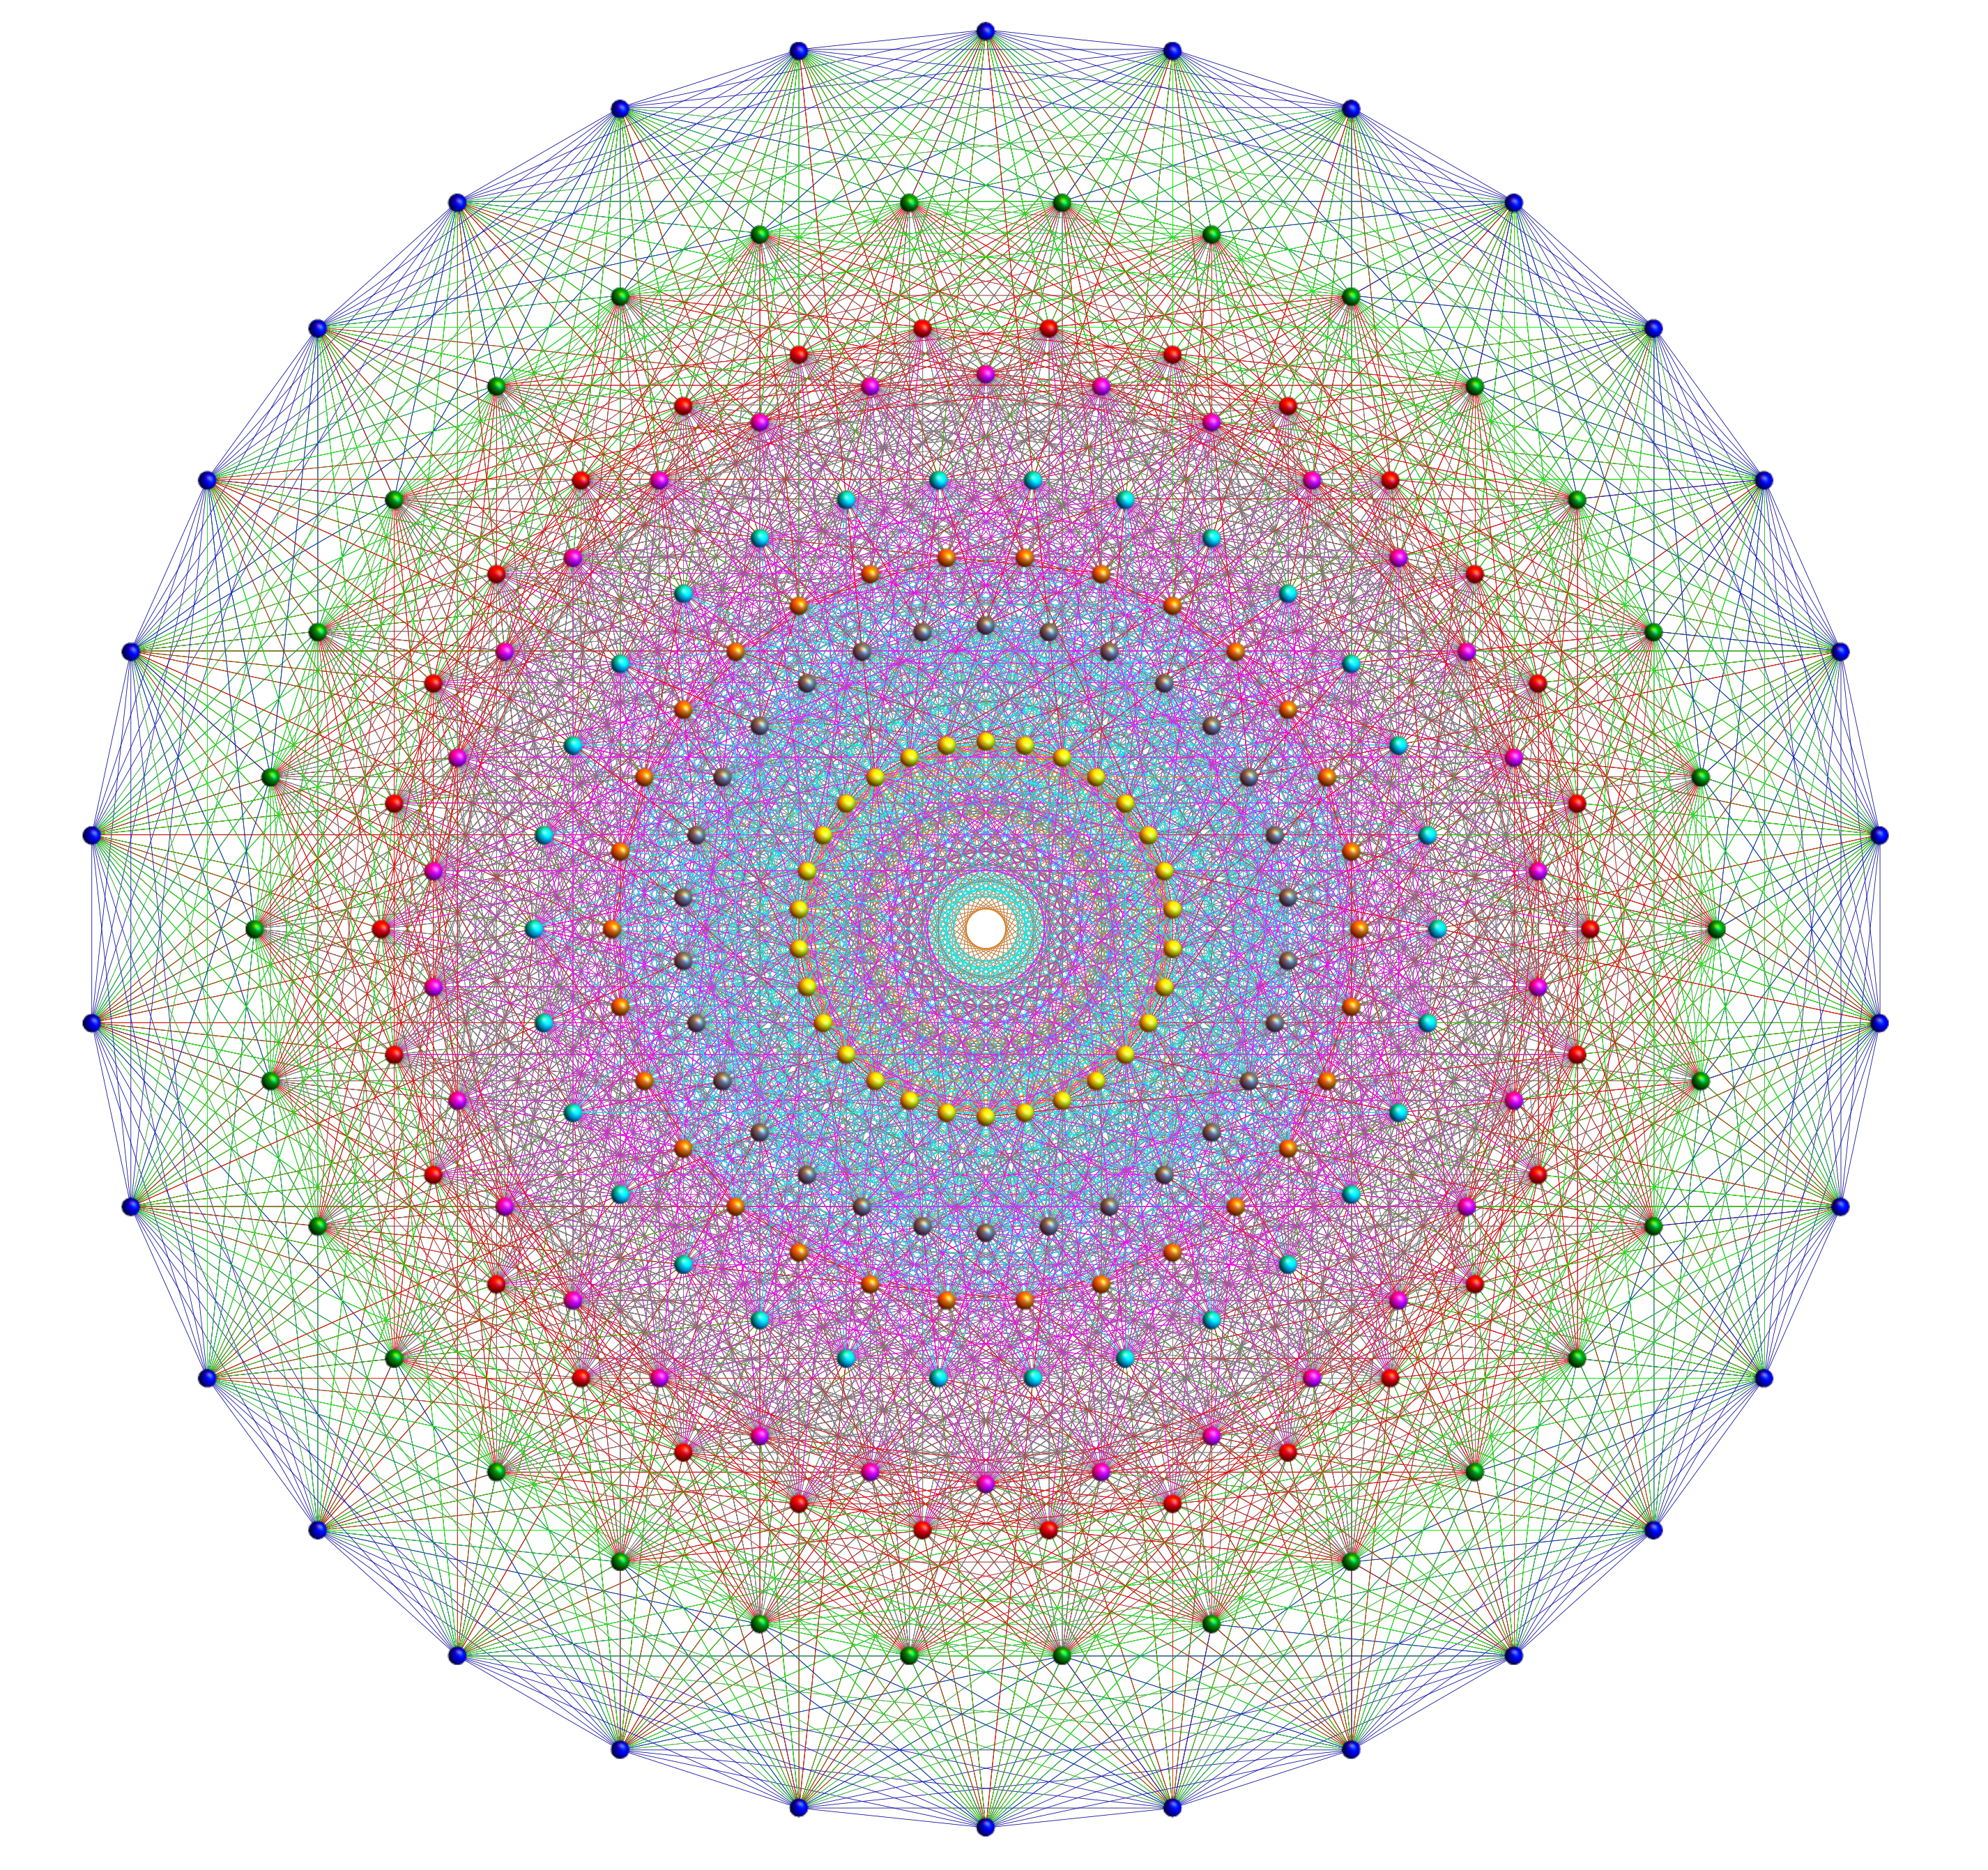
\includegraphics[width=.8\columnwidth]{front.jpeg}
\end{figure}

\newpage
\tableofcontents 
\newpage
\section{Teoria dei gruppi}
\subsection{Il gruppo degli automorfismi}
\begin{lemma}
	Siano $H,G$ due gruppi ciclici; un omomorfismo $\varphi : G \to H$ \`e univocamente determinato da come agisce su un generatore di $G$.
	\begin{proof}
		Sia $g_0\in G$ tale che $\langle g_0 \rangle = G$ e sia $\varphi (g_0) = \overline{h}\in H$.
		Per $g \in G$ generico, per cui $g_0^k = g$ per qualche intero $k$, si ha:
		\[
		\varphi (g) = \varphi (g_0^k) = \varphi (g_0)^k = \overline{h}^k
		\] 
		Cio\`e tutti gli elementi di $\operatorname{Im} \varphi $ sono esprimibili come potenze di $\overline{h}$.
	\end{proof}
\end{lemma}
\begin{osservazione}
Non ogni scelta di $\overline{h} \in H$ \`e ammissibile, ma bisogna rispettare l'ordine di $g_0$.
Se $g_0^n = e_G$, allora $e_H = \varphi (g_0^n) = \varphi (g_0)^n = \overline{h}^n$. Questa condizione, impone che $\operatorname{ord}(\overline{h})  \mid \operatorname{ord}(g_0) $.
\end{osservazione}
\begin{definizione}
	[Gruppo degli automorfismi]
	Sia $G$ un gruppo; si definisce il gruppo dei suoi automorfismi come
	\[
	\operatorname{Aut} (G) = \left\{ f: G \to G  \mid f \text{ \`e un isomorfismo di gruppi} \right\} 
	\] 
\end{definizione}
\begin{esempio}
	Si calcola $\operatorname{Aut} (\mathbb{Z})$. 
	\begin{svolgimento}
		Il gruppo $(\mathbb{Z},+)$ \`e ciclico, quindi un omomorfismo \`e determinato in base a come agisce su un generatore.
		Prendendo, per esempio $1$, si definisce $q_a :\mathbb{Z}\to \mathbb{Z} $ tale che $ q_a (1 ) = a$; perch\'e $\langle q_a(1) \rangle = \mathbb{Z}$\footnote{Richiesto dal fatto che $q_a$ sia suriettivo.}, \`e necessario che $a$ sia un generatore di $\mathbb{Z}$, perci\`o sono ammessi $a = \pm 1$. 
		In questo caso, $\operatorname{Aut} (\mathbb{Z})=\left\{ \pm \operatorname{Id} _{\mathbb{Z}}  \right\} \cong \left(\mathbb{Z} / 2\mathbb{Z}, +\right) $.
	\end{svolgimento}
\end{esempio}
\begin{teorema}
$\operatorname{Aut} (\mathbb{Z} / m \mathbb{Z}) \cong (\mathbb{Z} / m \mathbb{Z})^*$.
\begin{proof}
	$(\mathbb{Z} / m\mathbb{Z}, + )$ \`e ciclico, quindi si stabilisce l'azione di $f:\mathbb{Z} / m\mathbb{Z}\to \mathbb{Z}/ m\mathbb{Z}$ su un generatore.
	Preso, allora, $\overline{k} \in \mathbb{Z} / m\mathbb{Z} $ tale che $\operatorname{gcd}(k,m) =1$ e scelto $f(\overline{k}) = \overline{a}$, si ha che $\langle f(\overline{k}) \rangle= \langle \overline{a} \rangle= \mathbb{Z} / m\mathbb{Z} \iff \operatorname{gcd}(a,m) =1	\iff \overline{a} \in \left(\mathbb{Z} / m\mathbb{Z}\right) ^* $.
\end{proof}
\end{teorema}
\begin{definizione}
	[Automorfismo interno]
	Sia $G$ un gruppo; si definisce $\phi _g :G\to G$, $ \forall g \in G$, come $\phi_g (x) =gxg^{-1} $ ed \`e detto \textit{automorfismo interno}. 
	L'insieme di questi automorfismi, al variare di $g \in G$, forma il gruppo
	\[
	\operatorname{Int} (G) = \left\{ \phi _g : G\to G  \mid g \in G \text{ e } \phi _g \text{ automorfismo interno} \right\} 
	\] 
\end{definizione}
\begin{prop}\label{intcar}
	Sia $G$ un gruppo; allora $\operatorname{Int} (G) \lhd \operatorname{Aut} (G)$ e $\operatorname{Int} (G) \cong G / Z(G)$.
	\begin{proof}
		$\operatorname{Int} (G)$ \`e un sottogruppo di $\operatorname{Aut} (G)$ perch\'e $\operatorname{Id} (x) = exe^{-1} = x  \Rightarrow \operatorname{Id} \in \operatorname{Int} (G)$.
		Inoltre, $\phi _g \circ \phi _h (x) = ghxh^{-1}g^{-1}=\phi _{gh} (x) \in \operatorname{Int} (G)$ e $\phi _{g^{-1} } \circ \phi _g (x) = x \Rightarrow \phi _g^{-1} = \phi _{g^{-1}} \in \operatorname{Int}(G)  $.

		\`E un sottogruppo normale perch\'e $\forall f \in \operatorname{Aut} (G)$, si ha 
		\[
		f \circ \phi _g \circ f^{-1}(x) = f \left(g f^{-1}(x) g^{-1}\right) =f(g) x f(g)^{-1} \in \operatorname{Int} (G)
		\] 
		Per finire, si definisce $\Phi : G \to \operatorname{Int} (G) $.
		Questo \`e un omomorfismo perch\'e $\Phi(gh)=\phi _{gh} = \phi _g\circ \phi _h = \Phi(g)\Phi(h)$.
		\`E, inoltre, suriettivo perch\'e ogni automorfismo interno \`e associato ad un elemento di $G$, cio\`e $\forall \phi _g \in \operatorname{Int} (G), \ \exists g \in G : \Phi(g) = \phi _g$.
		Allora, la tesi deriva dal I teorema di omomorfismo, visto che $\operatorname{Ker} \Phi = Z(G)$.
	\end{proof}
\end{prop}
\begin{osservazione}\label{ossnorm}
	$H \lhd G \iff \phi _g(H) = H, \ \forall \phi _g \in \operatorname{Int} (G)$.
	\begin{proof}
Per ogni elemento di $\operatorname{Int} (G)$, si ha $\phi _g (H) = H \iff gH g^{-1} = H \iff H \lhd G$.
	\end{proof}
	\end{osservazione}
\begin{definizione}
	[Sottogruppo caratteristico]
	Sia $G$ un gruppo e $H < G$. Si dice che $H$ \`e \textit{caratteristico} se \`e invariante per automorfismo, cio\`e $\forall f \in \operatorname{Aut} (G), \ f(H) = H$.
\end{definizione}
\begin{corollario}
	Sia $G$ un gruppo; per la proposizione \ref{intcar} e l'osservazione \ref{ossnorm} se $H$ \`e caratteristico, allora $H \lhd G$.
\end{corollario}
\noindent Il viceversa \`e falso, cio\`e normale $\not\Rightarrow $ caratteristico; infatti, in $\mathbb{Z} / 2\mathbb{Z} \times  \mathbb{Z} / 2\mathbb{Z}$, il sottogruppo $\langle (1,0) \rangle$ \`e normale, ma non caratteristico perch\'e l'automorfismo che scambia le coordinate \`e tale per cui $\langle (1,0) \rangle\mapsto \langle (0,1) \rangle\neq \langle (1,0) \rangle$.
\subsection{Azioni di gruppo}
\begin{definizione}
	[Azione]
	Sia $G$ un gruppo; un'azione di $G$ su un insieme $X$ \`e un omomorfismo
	\[
	\gamma : 
	\begin{array}
		{c c c}
		G &\longrightarrow & S(X) = \left\{ f : X \to X  \mid f \text{ biettiva} \right\} \\
		g & \longmapsto & \psi _g : \psi_g(x) = g \cdot x
	\end{array}
	\] 
\end{definizione}
\begin{esempio}
Sia $G = \left\{ z \in \mathbb{C}^*  \mid  \lvert z \rvert =1 \right\} \cong S^1$ la circonferenza unitaria e $X = \mathbb{R}^2$.
Un'azione di $G$ su $X$ \`e una rotazione definita da $\gamma(z) = R(\operatorname{arg} z)$.
Questa \`e un omomorfismo perch\'e $\gamma(zw) = R(\operatorname{arg} zw)  = R(\operatorname{arg} z +  \operatorname{arg} w) = R(\operatorname{arg} z) R(\operatorname{arg} w)= \gamma(z) \gamma(w)$.
\end{esempio}
\noindent Un'azione $\gamma$ di $G$ su $X$ definisce, proprio su $X$, una relazione di equivalenza definita da 
\begin{equation}
	x \sim _\gamma y \iff x=\psi _g(y)=g \cdot y, \text{ con } x,y \in X
\end{equation}
La relazione di equivalenza \`e ben definita perch\'e le $\psi _g$ sono mappe biettive.
\begin{definizione}
	[Orbita]
	Sia $\gamma :G \to S(X)$ un'azione di $G$ gruppo su $X$. Dato $x \in X$, la sua classe di equivalenza rispetto alla relazione $\sim _\gamma$ \`e detta \textit{orbita} ed \`e indicata con $\operatorname{Orb} (x) = \left\{ g \cdot  x  \mid g \in G\right\} $.
\end{definizione}
\noindent Ricordando che una relazione di equivalenza fornisce una partizione dell'insieme su cui \`e definita, si ha:
\begin{equation}
	X = \bigsqcup_{x \in R} \operatorname{Orb} (x)
\end{equation}
con $R$ insieme dei rappresentati di tutte le orbite.
Se, poi, $X$ ha cardinalit\`a finita, allora:
\begin{boxenv}[]
\begin{equation}
	\lvert X \rvert  = \sum_{x \in R}^{} \lvert \operatorname{Orb} (x) \rvert 
\end{equation}
\end{boxenv}
\begin{definizione}
	[Stabilizzatore]
	Sia $\gamma: G \to S(X)$ un'azione di $G$ su $X$; allora per ogni $x \in X$, si definisce l'insieme 
	\[
	\operatorname{Stab} (x) = \left\{ g \in G  \mid g \cdot  x = x \right\} < G 
	\] 	
\end{definizione}
\begin{lemma}\label{l111}
Se due elementi di un'orbita sono uguali, allora appartengono alla stessa classe di equivalenza di $G / \operatorname{Stab} (x)$.
\begin{proof}
	Se $g \cdot x, \ h\cdot x \in \operatorname{Orb} (x)$ sono uguali, allora $x =h^{-1} g \cdot x $, cio\`e $h^{-1} g \in G$ lascia invariato $x$, quindi \`e in $\operatorname{Stab} (x)$.
	Da questo segue che $h \operatorname{Stab} (x) = h h^{-1} g \operatorname{Stab} (x) = g \operatorname{Stab} (x)$.
\end{proof}
\end{lemma}
\begin{teorema}[Teorema di orbita-stbilizzatore]\label{osth}
	Esiste una mappa biettiva $\Gamma : \operatorname{Orb} (x) \to G / \operatorname{Stab} (x)$ tale che $\Gamma(g \cdot x) = g \operatorname{Stab} (x)$.
	\begin{proof}
		$\Gamma$ \`e iniettiva come diretta conseguenza del lemma \ref{l111} ed \`e suriettiva perch\'e $\forall g \operatorname{Stab} (x) \in G / \operatorname{Stab} (x), \exists g\cdot x \in \operatorname{Orb} (x)$ tale che $\Gamma(g\cdot x) = g \operatorname{Stab} (x)$.
		Segue che $\lvert \operatorname{Orb} (x)  \rvert = \lvert G \rvert / \lvert \operatorname{Stab} (x) \rvert $.
	\end{proof}
\end{teorema}
\begin{osservazione}
Si osserva che, per il teorema di orbita-stabilizzatore, la cardinalit\`a di un'orbita indica il numero di classi laterali dello stabilizzatore nel gruppo che compie l'azione, cio\`e il teorema di orbita-stabilizzatore si pu\`o riscrivere come $\lvert \operatorname{Orb} (x) \rvert = [G: \operatorname{Stab} (x)] = \lvert G / \operatorname{Stab} (x) \rvert = \lvert G \rvert / \lvert \operatorname{Stab} (x) \rvert $.
\end{osservazione}

\noindent Un caso notevole di azione \`e il coniugio: per $X=G$, si definisce $\gamma : G \to \operatorname{Int} (G) \subset S(G)$.
Le orbite indotte da questa azione sono dette \textit{classi di coniugio} e si indicano con $\operatorname{cl} (x)$, mentre lo stabilizzatore \`e detto \textit{centralizzatore} e si indica con:
\begin{equation}
	Z(x) = \left\{ g \in G  \mid g \cdot x = gxg^{-1} = x \right\} 
\end{equation}
Come conseguenza del teorema di orbita-stabilizzatore (\ref{osth}), si ha:
\begin{equation}
	\lvert G \rvert  = \lvert \operatorname{cl} (x)  \rvert  \lvert Z(x) \rvert , \ \forall x \in G
\end{equation}
\begin{prop}
	Sia $G$ un gruppo e $\gamma$ l'azione di coniugio su di esso; allora
	\[
	\bigcap_{x \in G} Z(x) = Z(G)
	\] 
	\begin{proof}
		Si ha $g \in Z(x), \ \forall x \iff gxg^{-1} =x , \ \forall x \in G \iff g \in Z(G)$.
	\end{proof}
\end{prop}
\begin{osservazione}
	[Centro di un sottogruppo]
	Sia $G$ un gruppo e $H < G$; allora il centro di $H$ \`e definito come 
	\[
	\bigcap_{x \in H}  Z(x) = Z(H)
	\] 
\end{osservazione}

\subsubsection{Azione di coniugio}


Si considera, ora, l'azione di coniugio di un gruppo $G$ su $X = \left\{ H \subseteq G  \mid H< G \right\} $ e $\gamma(g) = \psi _g$ tale che $\psi_g (H) = gH g^{-1} $. 
Questa \`e un'azione ed \`e ben definita.
\begin{proof}
	Per dimostrare che \`e un'azione, si deve mostrare che la mappa $g \stackrel{\gamma}{\mapsto} \psi _g$ \`e un omomorfismo e che $\psi _g : X \to X$ sia biettiva.

	Si nota che $g \stackrel{\gamma}{\mapsto} \psi _g$ \`e un omomorfismo perch\'e $\psi _{g_1g_2} (H) = g_1g_2Hg_2^{-1}g_1^{-1} = \psi _{g_1} \circ \psi _{g_2} (H)$, cio\`e $g_1g_2\mapsto \psi _{g_1} \psi _{g_2} $.
	Inoltre, $\psi _g:X\to X$ \`e biettiva perch\'e $\exists \psi ^{-1} _g = \psi _{g^{-1}} : \psi _{g^{-1}} \circ \psi _g (H) = H $.

	Per mostrare che \`e ben definita, si fa vedere che effettivamente $\forall g, \psi_g$ mappa un sottogruppo di $G$ in un altro sottogruppo, cio\`e che $gHg^{-1} < G$.
	Intanto, $e \in gHg^{-1} $ perch\'e $H < G \Rightarrow  e \in H \Rightarrow geg^{-1}=e$; poi, $(ghg^{-1})(gh'g^{-1}) = ghh'g^{-1} \in g H g ^{-1}$ e $h^{-1} \in H \Rightarrow \exists (ghg^{-1} )^{-1} = g h^{-1}g^{-1}\in gHg^{-1}$ elemento inverso.
\end{proof}
\noindent Lo stabilizzatore di questa azione \`e detto \textit{normalizzatore}, in quanto \`e definito come tutti elementi di $G$ rispetto a cui $H$ \`e normale: 
\begin{equation}
	N_G(H) = \operatorname{Stab} (H) = \left\{ g \in G  \mid g H g^{-1}= H \right\} 
\end{equation}
Infine, l'orbita \`e l'insieme (classe di equivalenza) di tutti i coniugati di un sottogruppo di $G$:
\begin{equation}
\operatorname{Orb} (H) = \left\{ gHg^{-1}  \mid  g \in G \right\} 
\end{equation}
Per il teorema di orbita-stabilizzatore (\ref{osth}), si ha:
\begin{equation}
	\lvert G \rvert  = \lvert N_G(H) \rvert \lvert \operatorname{Orb} (H) \rvert 
\end{equation}
da cui si ricava anche che $H \lhd G \iff N_G(H) = G \iff \operatorname{Orb} (H) = \left\{ H \right\} $.
\subsubsection{Formula delle classi}

Si ricorda che le orbite definite da un'azione di un gruppo $G$ su un insieme $X$ formano una partizione di $X$ stesso, in quanto sono delle classi di equivalenza.
Se $\lvert X \rvert < \infty$, si ha:
\begin{equation}\label{ossclass}
\lvert X \rvert  = \sum_{x \in R}^{} \lvert \operatorname{Orb} (x) \rvert = \sum_{x \in R}^{} \frac{\lvert G \rvert }{\lvert \operatorname{Stab} (x) \rvert } = \sum_{x \in R'}^{} 1 + \sum_{x \in R \setminus R '}^{} \frac{\lvert G \rvert }{\lvert \operatorname{Stab} (x) \rvert }
\end{equation}
con $R$ insieme dei rappresentanti delle orbite e $R'$ insieme dei rappresentati delle orbite tali che $\operatorname{Orb} (x) = \left\{ x \right\} $, cio\`e degli elementi invarianti sotto l'azione di $G$. 
\begin{teorema}
	[Formula delle classi]
	Sia $\gamma:G \to S(G)$ l'azione di coniugio di un gruppo $G$ su un insieme $X$; allora:
	\begin{equation*}
		\lvert G \rvert  = Z(G) + \sum_{x \in R \setminus Z(G)}^{} \frac{\lvert G \rvert }{\lvert Z(x) \rvert }
	\end{equation*}
	\begin{proof}
		Segue per quanto appena detto e dall'osservazione che
		\[
		R' = \left\{ x \in R  \mid \operatorname{Orb} (x) = x \right\} = \left\{ x \in R  \mid gxg^{-1} = x \right\} = Z(G)
		\] 
		Visto che ogni orbita del genere contiene un solo elemento, i rappresentanti delle orbite sono esattamente tutti gli elementi di $Z(G)$, cio\`e un elemento $x \in Z(G)$ non pu\`o essere contenuto in nessun'altra orbita, se non nel singoletto $\left\{ x \right\} $.
		Perci\`o, la relazione in eq. \ref{ossclass}, avendo $X=G$, conferma la tesi.
	\end{proof}
\end{teorema}
\subsection{I p-gruppi}
\begin{definizione}
	[p-gruppo]
	Sia $p \in \mathbb{Z}$ un numero primo; allora si dice che $G$ \`e $p$-gruppo se $\lvert G \rvert = p^n$, per qualche $n \in \mathbb{N}$.
\end{definizione}
\begin{prop}\label{pnb}
	Il centro di un $p$-gruppo \`e non-banale.
	\begin{proof}
		Per la formula delle classi, si ha:
		\[
		p^n = \lvert Z(G) \rvert  + \sum_{x \in R \setminus Z(G)}^{} \frac{\lvert G \rvert }{\lvert Z(x) \rvert }
		\] 
		Se $\lvert Z(G) \rvert  = p^n$, la tesi \`e verificata, altrimenti $\exists x \in R \setminus Z(G)$, quindi tale che $Z(x) \subsetneq G$; allora, per qualche intero $k>0$, si ha $\lvert G \rvert / \lvert Z(x) \rvert = p^k$, da cui
		\[
		\lvert Z(G) \rvert =p^n - \sum_{x \in R \setminus Z(G)}^{} p^k\implies p  \mid \lvert Z(G) \rvert 
		\] 
		Visto che $e \in Z(G)$, deve risultare $\lvert Z(G) \rvert \ge 1$, da cui $\lvert Z(G) \rvert = p^s$, per qualche intero $s > 1$.
	\end{proof}
\end{prop} 
\begin{lemma}\label{GZGciffban}
	Vale $G / Z(G)$ ciclico $\iff G$ \`e abeliano.
	\begin{proof}
		Sia $G / Z(G)$ ciclico e sia $x_0 Z(G)$ il suo generatore.
		Date due classi laterali distinte $xZ(G), yZ(G) \in G / Z(G)$ e visto che $x_0Z(G)$ genera, si avr\`a $x_0^m Z(G)= x Z(G)$ e $x_0^nZ(G) = yZ(G)$, ossia, per $z,w \in Z(G)$, $x = x_0^m z,\ y = x_0^n w$. 
		Allora:
		\[
			 xy = x_0^m z x_0^n w = x_0^m x_0^n zw = x_0^n wx_0^m z = yx
		\] 
	Essendo questo valido per $x,y \in G$ generiche, si \`e dimostrata l'implicazione verso destra.

	Per l'implicazione inversa, sia $G$ abeliano; allora $Z(G) = G$ e $G / Z(G) = \left\{ e \right\} $, che \`e ovviamente ciclico.
	\end{proof}
\end{lemma}
\begin{prop}
	Un gruppo di ordine $p^2$ \`e abeliano.
	\begin{proof}
		Sia $G$ un $p$-gruppo tale che $\lvert G \rvert  = p^2$. Per mostrare che \`e abeliano, si fa vedere che $Z(G) = G$, ossia $\lvert Z(G) \rvert  = p^2$.
		Per la proposizione \ref{pnb}, si pu\`o avere solamente $\lvert Z(G) \rvert = p$, oppure $\lvert Z(G) \rvert = p ^2$.
		Se, per assurdo, fosse $\lvert Z(G) \rvert =p$, allora $\lvert G \rvert / \lvert Z(G) \rvert = p$, quindi $G / Z(G)$ avrebbe ordine primo e, quindi, sarebbe ciclico; per il lemma precedente (\ref{GZGciffban}), per\`o, questo \`e assurdo perch\'e risulterebbe anche abeliano al contempo, ma senza avere $\lvert Z(G) \rvert  = \lvert G \rvert $.
		Quindi deve essere $\lvert Z(G) \rvert  = p^2 = \lvert G \rvert \Rightarrow Z(G) = G$, da cui $G$ \`e abeliano.
	\end{proof}
\end{prop}
\subsection{Teoremi di Cauchy e Cayley}
\begin{lemma}[Teorema di Cauchy abeliano]\label{cab}
	Sia $p$ un primo e $G$ un gruppo abeliano finito; se $p  \mid  |G|$, allora $\exists x \in G : \operatorname{ord}(x) =p$.
	\begin{proof}
		Sia $\lvert G \rvert = pn$; si procede per induzione su $n$.
		Il passo base \`e ovvio: se $\lvert G \rvert =p$, allora \`e ciclico e, quindi, contiene un elemento di ordine $p$.

		Per il passo induttivo, si suppone che la tesi sia vera per ogni $m < n$ e si dimostra per $n$.

		Sia, allora $\lvert G \rvert  = pn$; sia, poi $y \in G, \ y\neq e$ tale che $\langle y \rangle= H < G$: per Lagrange, $\lvert G \rvert  = \lvert G / H \rvert  \lvert H \rvert $.
		Allora, se $p  \mid \lvert G \rvert \Rightarrow  p  \mid \lvert H \rvert $, oppure $ p   \mid \lvert G / H \rvert $.
		\begin{itemize}
			\item Se $p  \mid \lvert H \rvert $, allora pu\`o essere $\lvert G \rvert  = \lvert H \rvert $, caso in cui $G = \langle y \rangle$ sarebbe ciclico e, quindi, avrebbe un elemento di ordine $p$\footnote{In questo caso, l'elemento di ordine $p$ sarebbe proprio $y^{p^{n-1} } \in G $; infatti, $(y^{p^{n-1} } )^p = y^{p^n} = e$, visto che $|G| = p^n$.}, oppure pu\`o essere $\lvert H \rvert  = pm < pn$, caso in cui l'elemento di ordine $p$ \`e presente per ipotesi induttiva.
			\item Se $p  \mid  \lvert G / H \rvert $, invece, allora $\lvert G / H \rvert = pm' < pn$ perch\'e $H$ contiene almeno due elementi, cio\`e $y$ ed $e$; per ipotesi induttiva, allora, esiste $zH \in G / H$ il cui ordine \`e $p$.
				Considerando la proiezione $\pi_H : G \to G / H$ tale che $x \mapsto xH$ e ricordando che \`e un omomorfismo, si ha che, per questo motivo, $\operatorname{ord}(zH)  \mid \operatorname{ord}(z)\Rightarrow \operatorname{ord}(z) = pk$; se $k = n$, allora $G$ \`e ciclico e $z^n$ ha ordine $p$, altrimenti, se $k<n$, si ha la tesi per induzione.
		\end{itemize}
	\end{proof}
\end{lemma}
\begin{teorema}
	[Teorema di Cauchy]
	Sia $p$ un numero primo e $G$ un gruppo finito; se $p  \mid |G|$, allora esiste $x \in G : \operatorname{ord}(x) = p $.
	\begin{proof}
		Sia $|G| = pn$, con $p$ primo e $n \in \mathbb{N}$; si procede per induzione su $n$.
		Se $n=1$, $|G| = p \Rightarrow G$ \`e ciclico, quindi $\exists x \in G : \langle x \rangle=G$ e $\operatorname{ord}(x) = p$.

		Per il passo induttivo, si assume che la tesi sia valida per ogni $ m < n$ e si dimostra per $n$.

Si nota che se $\exists  H < G$ tale che $p  \mid  \lvert H \rvert $, allora $|H|=pm , \ m < n \Rightarrow \exists x \in H$ tale che $\operatorname{ord}(x) =p$ per ipotesi induttiva.
Si assume, dunque, che non esista alcun sottogruppo di $G$ il cui ordine sia divisibile per $p$.
Per la formula delle classi
\[
pn - \sum_{x \in R\setminus Z(G)}^{} \frac{\lvert G \rvert }{|Z(x)|} = \lvert Z(G) \rvert 
\] 
Ora, visto che $Z(x) < G \Rightarrow p \not  \mid Z(x)$, quindi si ha la certezza che, essendo $p  \mid |G| = |Z(x)| |G|/|Z(x)|$, $p$ divide $|G|/|Z(x)|$. 
Allora $p  \mid  |Z(G)|$, per cui $Z(G) =G$; infatti, se cos\`i non fosse, sarebbe un sottogruppo proprio di $G$ e $p$ non lo potrebbe dividere, il che \`e assurdo.

Da questo, segue che $G$ \`e abeliano, quindi la tesi segue dal teorema di Cauchy per gruppi abeliani (lemma \ref{cab}).
	\end{proof}
\end{teorema}
\begin{prop}\label{tgen}
Siano $H,K < G$; allora $HK < G \iff HK = KH$ e $\lvert HK \rvert = \lvert H \rvert \lvert K \rvert / \lvert H \cap K \rvert $.
\begin{proof}
Per la prima parte, \`e sufficiente osservare che per $hk \in HK$, l'elemento neutro $(hk)^{-1} = k^{-1} h^{-1} $ sta in $HK$ se e solo se $HK = KH$, e, allo stesso modo, il prodotto \`e chiuso cio\`e $hkh'k' = hh''k''k' \in HK$ solamente se $HK = KH$ cos\`i da poter trovare un elemento di $HK$ che sia uguale a $kh'\in KH$ che compare in tale prodotto.

La seconda parte, invece, si verifica considerando l'applicazione $\gamma: H \times K\to HK$ tale che $\gamma((h,k)) = hk$, che \`e evidentemente suriettiva; inoltre, se $s \in H \cap K$, allora $(hs,s^{-1}k) \in H \times K\Rightarrow \gamma ((hs,s^{-1}k)) = hk$, il che vuol dire che $\forall hk \in HK$, si trovano $|H\cap K|$ coppie in $H \times K$ che hanno immagine $hk$, da cui la tesi.
\end{proof}
\end{prop}
\begin{boxenv}[Classificazione dei gruppi di ordine 6]
Sia $G$ un gruppo di ordine $6$; per Cauchy, allora, esistono $x,y \in G$ tali che $\operatorname{ord}(x) = 2$ e $\operatorname{ord}(y) =3$. 
Se $G$ \`e abeliano, poi, si ha $\operatorname{ord}(xy) = 6$\footnote{Si dimostra per calcolo diretto; per esempio: $(xy)^3 = xyxyxy=xx x yyy=x$.}, quindi $G = \langle xy \rangle\cong \mathbb{Z}/ 6\mathbb{Z}$.

Se, invece, $G$ non \`e abeliano, si considera il sottogruppo $\langle x,y \rangle$ e si considera anche l'insieme $\langle x \rangle\langle y \rangle$ che, in generale, non \`e un sottogruppo.

Applicando la proposizione precedente (\ref{tgen}), si ha che $\lvert \langle x,y \rangle \rvert = (3 \cdot 2) / 1= 6$\footnote{L'intersezione \`e solo l'unit\`a perch\'e i due elementi hanno ordini diversi, quindi generano gruppi disgiunti.}, da cui $G = \langle x \rangle\langle y \rangle$, con $\langle x \rangle= \left\{ e,x \right\} $ e $\langle y \rangle= \left\{ e,y,y^2 \right\} $, quindi $G = \left\{ e , x ,y, xy,y^2 , xy^2 \right\} $.

Per finire, si mostra che $G \cong S_3$. 
Per farlo, si definisce $\phi :G \to S_3=\left\{ e,\tau ,\rho ,\tau \rho ,\tau ^2,\rho \tau ^2 \right\} $ tale che $\phi (x) = \rho $ e $\phi (y) = \tau $, con $\tau =(1,2,3)$ e $\rho = (1,2)$.
Questa mappa \`e suriettiva per costruzione, quindi \`e biettiva per questioni di cardinalit\`a; inoltre, \`e un omomorfismo, da cui segue la tesi.
\end{boxenv}

\begin{teorema}
	[Teorema di Cayley]
	Sia $G$ un gruppo; allora $G$ \`e isomorfo a un sottogruppo di $S(G)$.
	In particolare, se $|G| = n$, allora $G$ \`e isomorfo a un sottogruppo di $S_n$.
	\begin{proof}
		Si definisce l'azione
		\[
		\phi : 
		\begin{array}
			{c c c}
			G & \longrightarrow & S(G)\\
			g & \longmapsto & \gamma_g
		\end{array}, \ \text{ tale che } \gamma_g(x) = g\cdot x
		\] 
		Questa \`e ben definita perch\'e $\gamma:G \to G$ \`e biettiva, infatti $\gamma_g(x) = \gamma_g(y) \iff g \cdot x = g \cdot y \iff x = y$ e $\forall y \in G , \ \exists \gamma_g(g^{-1} \cdot y) = y $, il che mostra che \`e rispettivamente iniettiva e suriettiva.
		Inoltre, $\phi $ \`e un omomorfismo (ovvio) ed \`e anche iniettiva perch\'e $\operatorname{Ker} \phi = \left\{ g \in G  \mid \phi _g = \phi _e \right\} = \left\{ g \in G  \mid g \cdot x = x \right\} = \left\{ e \right\}$.
		Da questo, segue che $S(G)$ contiene una copia isomorfa a $G$.
	\end{proof}
\end{teorema}
\subsection{Commutatore e gruppo derivato}


\begin{definizione}
	Sia $G$ un gruppo e $S \subset G$ un suo sottoinsieme; allora $\langle S \rangle$ \`e il pi\`u piccolo sottogruppo di $G$ contenente anche $S$.
\end{definizione}
\begin{prop}
	Dato $G$ un gruppo e $S \subset G$ un suo sottoinsieme, vale la relazione
	\[
	\langle S \rangle= \left\{ s_1s_2 \ldots s_k  \mid k \in \mathbb{N}, \ s_i \in S \cup S^{-1} \right\} = X
	\] 
	con $S^{-1}= \left\{ s^{-1}  \mid  s \in S \right\} $.
	\begin{proof}
		Per definizione
		\[
			\langle S \rangle= \bigcap_{\substack{H < G \\ S \subset H}} H
		\] 
		Questa scrittura \`e ben definita perch\'e l'intersezione di gruppi \`e ancora un gruppo e, in questo modo, si ha il gruppo pi\`u piccolo contenente $S$; se cos\`i non fosse, ne esisterebbe uno pi\`u piccolo ancora, che, per\`o, farebbe parte dell'intersezione e sarebbe assurdo.

		Ora, per quanto detto sopra, $S$ \`e contenuto in tutti i gruppi la cui intersezione genera $\langle S \rangle$, quindi anche $S^{-1} $ deve essere contenuto in tali sottogruppi di $G$.
		Segue che $S,S^{-1}\subset H \Rightarrow X \subset H, \ \forall H < G$ e $S \subset H$, quindi $X \subset \bigcap H = \langle S \rangle$.

		Allo stesso tempo, $X$ \`e evidentemente un sottogruppo di $G$ e contiene $S$ per costruzione, quindi $X \supset \langle S \rangle$, da cui la tesi.
	\end{proof}
\end{prop}
\begin{definizione}
	[Commutatore]
	Sia $G$ un gruppo; dati $g,h \in G$, il loro \textit{commutatore} \`e definito come
	\[
		[g,h] = ghg^{-1} h^{-1}
	\] 
\end{definizione}
\begin{definizione}
	[Gruppo derivato]
	Dato un gruppo $G$, si definisce \textit{gruppo dei commutatori}, o \textit{derivato} di $G$, il gruppo 
	\[
		G ' = \langle [g,h]  \mid g,h \in G \rangle = [G:G]
	\] 
\end{definizione}
\noindent Ora si caratterizza il gruppo derivato.
Intanto, si ricorda che $\langle S \rangle$ \`e abeliano $\iff \forall s_1,s_2\in S , \  s_1s_2=s_2s_1$, $\langle S \rangle$ \`e normale $\iff \forall g \in G, \forall s \in S, \ gsg^{-1} \in \langle S \rangle$ e, infine, $\langle S \rangle$ \`e caratteristico $\iff \forall f \in \operatorname{Aut} (G) ,\ \forall s \in S$ si ha $f(s) \in S$.
Applicando queste alla definizione di commutatore, si ottiene la seguente.
\begin{prop}\label{propderiv}
	[Propriet\`a del derivato]
	Sia $G$ un gruppo e $G'$ il suo derivato; allora:
	\begin{enumerate}[(a).]
		\item $G ' = \left\{ e \right\}  \iff G$ \`e abeliano;
		\item $G' \lhd G$;
		\item $G'$ \`e caratteristico in $G$;
		\item dato $H \lhd G$, se $G / H$ \`e abeliano, allora $G' \subset H$.
	\end{enumerate}
	\begin{proof}
		La (a) \`e immediata perch\'e $G' = \left\{ e \right\} \iff \forall g_1,g_2 \in G, \ [g_1,g_2] = e $, cio\`e $g_1$ e $g_2$ commutano, da cui $G$ abeliano.

		Per la (b), $\forall x \in G, \ \forall g,h \in G $, si ha 
		\[
			\begin{split}
				x[g,h]x^{-1}  &= xghg^{-1}h^{-1}x^{-1}= xgx^{-1}xhx^{-1}xg^{-1}x^{-1}xh^{-1}x^{-1}\\
					      &=[xgx^{-1}, xhx^{-1}] \in G'
			\end{split}
		\] 
	Per la (c), si nota che $\forall f \in \operatorname{Aut} (G), \ \forall g,h \in G$, si ha:
	\[
		f([g,h]) = f(ghg^{-1}h^{-1}) = f(g) f(h) f(g)^{-1} f(h)^{-1} = [f(g), f(h)] \in G'
	\] 
	Infine, per la (d), se $H \lhd G$ e $G / H$ \`e abeliano, si ha $\forall x,y \in G$
	\[
		xHyH =yH xH\Rightarrow xyH = yxH \implies x^{-1}y^{-1}xy \in H \Rightarrow [x,y] \in H
	\] 
	da cui $H \supset G' $.
	\end{proof}
\end{prop}
\begin{corollario}
	Sia $G$ un gruppo e $G'$ il suo derivato; allora $G / G'$ \`e sempre abeliano ed \`e chiamato \textit{abelianizzazione} di $G$, nel senso che \`e il pi\`u grande quoziente abeliano di $G$.
	\begin{proof}
		Si mostra che $G / G'$ \`e sempre abeliano. 
		Siano, quindi $gG', hG' \in G / G'$ due classi laterali; allora si osserva che
		\[
			(gG') (hG') = ghG' = hg [g^{-1},h^{-1}] G' = hg G'
		\] 
		visto che $g^{-1}h^{-1}gh=[g^{-1},h^{-1}] \in G'$.
		Allora, dalla propriet\`a (d) della precedente proposizione (\ref{propderiv}), si ha $G' \subset H =G'$, cio\`e in questo caso si ha l'inclusione nell'insieme pi\`u piccolo, ovvero proprio $G'$. 
		Questo vuol dire che $G /G'$ \`e il quoziente con pi\`u elementi che sia abeliano perch\'e ottenuto tramite quoziente con $G'$, che \`e l'insieme pi\`u piccolo che soddisfa la propriet\`a\footnote{Per controposizione, se $G'\not\subset H\implies G/H$ non abeliano.}.
	\end{proof}
\end{corollario}
\subsection{Gruppi diedrali}


\end{document}
